\documentclass[table,dvipsnames]{beamer}
\mode<presentation>{
	\usetheme{Madrid}
	\setbeamercolor{title}{fg=Black,bg=Blue!15}
	\setbeamercolor{frametitle}{fg=Black,bg=Blue!15}
	\setbeamercolor{block title}{fg=Black,bg=Blue!15}
	\setbeamercolor{block}{fg=Black,bg=Blue!10}
}

\usepackage{graphicx}
\usepackage{booktabs}
\usepackage{xcolor}
\usepackage{multirow}
\usepackage{minted}
\usepackage[
type={CC},
modifier={by-sa},
version={4.0},
]{doclicense}

\definecolor{LightGray}{gray}{0.9}

\title[Audiometri]{Technical Aspect: Audiometri}
\author{}
\institute[VibrasticLab : \ccbysa]{
	Achmadi ST MT
}
\date{}

\begin{document}	
	\begin{frame}
		\titlepage
	\end{frame}

	\begin{frame}[fragile]
		\frametitle{Tone Array}
		
		\begin{exampleblock}{}
			\begin{minted}[frame=lines,framesep=2mm,fontsize=\tiny,bgcolor=LightGray]{c}
#define I2S_BUFF_SIZE 512 // Default audio array size
#define DEFAULT_ATTEN 0.01 // Array attenuation
			\end{minted}
		\end{exampleblock}
		
		\begin{exampleblock}{}
			\begin{minted}[frame=lines,framesep=2mm,fontsize=\tiny,bgcolor=LightGray]{c}
buffsize = (uint16_t) I2S_BUFF_SIZE/freq; // Buffer size define the frequency

for(i=0;i<buffsize;i++){
	
	// Y = A * x * sin (2*pi*f)

	ysin = DEFAULT_ATTEN*ampl*32767*sin(2*3.141592653589793*((double)i/(double)buffsize));
	
	if(ysin >= 0) i2s_tx_buf[i]=ysin; // positive y
	if(ysin < 0) i2s_tx_buf[i]=ysin+65535; // negative y
}

// apply array size as frequency scaling
i2scfg.size = buffsize;
			\end{minted}
		\end{exampleblock}
	
	\end{frame}

	\begin{frame}[fragile]
		\frametitle{Tone Scaling by Half}
		
		\begin{exampleblock}{}
			Prepared output scale in each frequency: 1, 2, 3, 4, 5, 6, 7, 8, 9.
		\end{exampleblock}
		
		\begin{exampleblock}{}
			\begin{minted}[frame=lines,framesep=2mm,fontsize=\tiny,bgcolor=LightGray]{c}
ysin_9 = 1 * ysin;
ysin_8 = 0.5 * ysin;
ysin_7 = 0.25 * ysin;
ysin_6 = 0.125 * ysin;
ysin_5 = 0.0625 * ysin;
ysin_4 = 0.0312 * ysin;
ysin_3 = 0.0156 * ysin;
ysin_2 = 0.0078 * ysin;
ysin_1 = 0.0039 * ysin;
			\end{minted}
		\end{exampleblock}
	\end{frame}

	\begin{frame}[fragile]
		\frametitle{Audio DAC (MAX98357A) Output Level}
		
	\begin{exampleblock}{}
		\centering
		Out = In + Gain + 2.1 dB
	\end{exampleblock}

	\begin{exampleblock}{}
		\begin{itemize}
			\item \textbf{Out}. Output signal level (dBV)
			\item \textbf{In}. Input signal level (dBFS)
			\item \textbf{Gain}. Selected Gain (dB)
		\end{itemize}
	\end{exampleblock}

	\begin{exampleblock}{}
		\begin{itemize}
			\item Gain is referenced to the full-scale output of the DAC,
which is 2.1dBV.
			\item The 0dBFS is referenced to 0dBV.
			\item Selected Gain is 3 dB in circuit design.
		\end{itemize}
	\end{exampleblock}

	\begin{exampleblock}{}
		\centering
		y dBV = x dBFS + 5.1 dB
	\end{exampleblock}

	\end{frame}

	\begin{frame}
		\frametitle{Actual Output}
		
		\begin{exampleblock}{}
			\begin{itemize}
				\item dBV output might be consistent, but actual output are not.
				\item Depends on each headphone's charateristic.
				\item Approach to use:
				\begin{enumerate}
					\item Testing actual tone for each scale in each frequency.
					\item Build polynomial model based on it.
					\item Put model on Data Viewer, not on chip (for flexibility).
				\end{enumerate}
			\end{itemize}
		\end{exampleblock}
	
		\begin{exampleblock}{}
			Example scale to dB each frequency for a Miniso headphone:
			\begin{gather}
y_{250} = 38.59 + 2.17*x + 0.63*x^2 - 0.03*x^3 \\
y_{500} = 39.31 + 2.67*x + 0.54*x^2 - 0.03*x^3
\\
y_{1000} = 42.89 + 2.65*x + 0.55*x^2 - 0.03*x^3
\\
y_{2000} = 37.62 + 0.63*x + 0.87*x^2 - 0.04*x^3
\\
y_{4000} = 40.3  - 2.85*x + 1.27*x^2 - 0.06*x^3
\\
y_{8000} = 43.34 - 3.19*x + 1.28*x^2 - 0.03*x^3
			\end{gather}
		\end{exampleblock}
	\end{frame}

	\begin{frame}
		\frametitle{Stop Test Condition}
		
		\begin{exampleblock}{}
			\begin{itemize}
				\item Reach lowest tone (scale 1)
				\item All possible chances (24) has been used up
				\item False turning point up to 5 times
			\end{itemize}
		\end{exampleblock}
	
		\begin{exampleblock}{}
			Turning point logic:
			\begin{itemize}
				\item if Up and previously Down, then False-Point increment by 1.
				\item if Down, previously Down, and then False-Point more than 3, then False-Point decrement by 1.
				\item if False-point is 5, test loop stop
			\end{itemize}
		\end{exampleblock}
	\end{frame}

	\begin{frame}[fragile]
		\frametitle{Test Result Sample (One Channel)}
	
		\begin{exampleblock}{}
			JSON text contains last scale (either by lowest or False-Points) and input record for each frequencies and channels.
		\end{exampleblock}
	
		\begin{exampleblock}{}
			\begin{minted}[frame=lines,framesep=2mm,fontsize=\tiny,bgcolor=LightGray]{json}
{"audiogram":{
 "ch_0":{
  "freq_0":{"freq": 0.625,"ampl":3,"record":[6,5,4,5,4,3,4,3,2,3,2,3,2,3,3,3,3,3,3,3,3,3,3,3]},
  "freq_1":{"freq": 1.250,"ampl":1,"record":[6,5,4,3,2,1,2,1,1,1,1,1,1,1,1,1,1,1,1,1,1,1,1,1]},
  "freq_2":{"freq": 2.500,"ampl":1,"record":[6,5,4,3,4,3,2,1,1,1,1,1,1,1,1,1,1,1,1,1,1,1,1,1]},
  "freq_3":{"freq": 5.000,"ampl":1,"record":[6,5,4,3,2,1,1,1,1,1,1,1,1,1,1,1,1,1,1,1,1,1,1,1]},
  "freq_4":{"freq":10.000,"ampl":1,"record":[6,5,4,3,2,1,1,1,1,1,1,1,1,1,1,1,1,1,1,1,1,1,1,1]},
  "freq_5":{"freq":20.000,"ampl":1,"record":[6,5,4,3,2,1,1,1,1,1,1,1,1,1,1,1,1,1,1,1,1,1,1,1]}},
 "ch_1":{
  "freq_0":{"freq": 0.625,"ampl":2,"record":[6,6,5,4,3,2,3,2,3,4,5,4,3,2,3,2,1,2,1,2,2,2,2,2]},
  "freq_1":{"freq": 1.250,"ampl":1,"record":[6,5,4,3,2,1,2,3,2,1,2,3,2,1,1,1,1,1,1,1,1,1,1,1]},
  "freq_2":{"freq": 2.500,"ampl":1,"record":[6,5,4,3,2,3,2,1,2,1,1,1,1,1,1,1,1,1,1,1,1,1,1,1]},
  "freq_3":{"freq": 5.000,"ampl":1,"record":[6,5,4,3,2,1,1,1,1,1,1,1,1,1,1,1,1,1,1,1,1,1,1,1]},
  "freq_4":{"freq":10.000,"ampl":1,"record":[6,5,4,3,2,1,1,1,1,1,1,1,1,1,1,1,1,1,1,1,1,1,1,1]},
  "freq_5":{"freq":20.000,"ampl":1,"record":[6,5,4,3,2,1,1,1,1,1,1,1,1,1,1,1,1,1,1,1,1,1,1,1]}}
 }
}
			\end{minted}
		\end{exampleblock}
	\end{frame}

	\begin{frame}[fragile]
		\frametitle{DataViewer (Windows/Linux)}
		
		\begin{exampleblock}{}
			Plot previous JSON data text re-calculated using headphone's polynomial model.
		\end{exampleblock}
	
		\begin{exampleblock}{}
			\begin{center}
				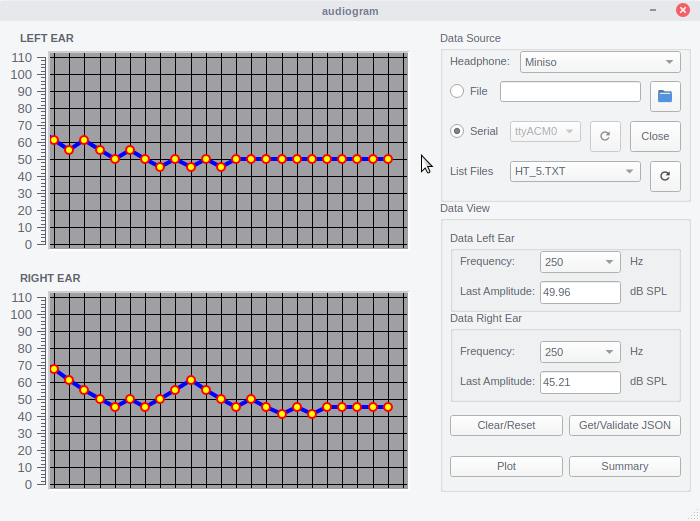
\includegraphics[width=200pt]{images/elbicare_qt5}
			\end{center}
		\end{exampleblock}
	\end{frame}

	\begin{frame}[fragile]
		\frametitle{DataViewer (Android/Web)}
		
		\begin{exampleblock}{}
			\begin{center}
				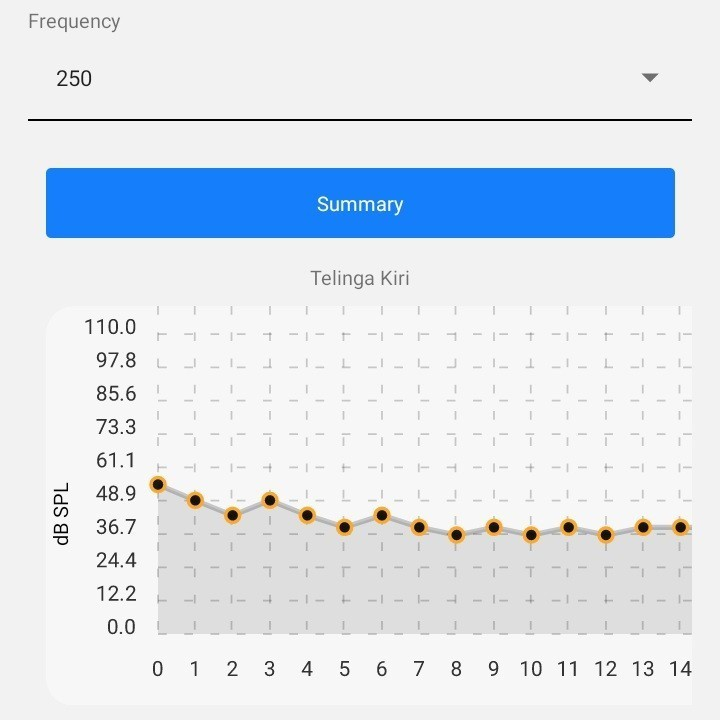
\includegraphics[width=200pt]{images/elbicare_android}
			\end{center}
		\end{exampleblock}
	\end{frame}

	\begin{frame}[fragile]
		\frametitle{ToDo: Click-Pop Suppression}
		
		\begin{exampleblock}{}
			Problems:
			\begin{itemize}
				\item Cause:
				\begin{itemize}
					\item No I2S CLK signal when MAX98357A shutted down causing sudden spike on chip's output when re-activated.
					\item MAX98357A has no internal volume ramped down routine when shutting down or lost I2S CLK signal.
				\end{itemize}
			
				\item Click-Pop not always heard on all kind of headphone.
			\end{itemize}
		\end{exampleblock}
	
		\begin{exampleblock}{}
			Approach:
			\begin{itemize}
				\item Zero-ing Audio Array before disable Audio transaction (Not always work everytime).
				\item Never stop data exchange so I2S CLK always present (Not work, causing output tone not single)
			\end{itemize}
		\end{exampleblock}
	\end{frame}

	\begin{frame}[fragile]
		\frametitle{ToDo: Low Tone Range}
		
		\begin{exampleblock}{}
			Problems: 
			\begin{itemize}
				\item Lowest measured tone is around 30dB SPL and can't be lower without unheard.
			\end{itemize}
		\end{exampleblock}
	
		\begin{exampleblock}{}
			Approach: None available for now
		\end{exampleblock}
	\end{frame}

	\begin{frame}[fragile]
		\frametitle{ToDo: Final Audiogram Result}
		
		\begin{exampleblock}{}
			Requirements: 
			\begin{itemize}
				\item Better understanding about dB HL in relation to dB SPL (or even also dBV and dBFS).
				\item Verify headphone's polynomial model tone output each scale in each frequency.
			\end{itemize}
		\end{exampleblock}
	\end{frame}

\end{document}
